\documentclass[a4paper,english,11pt,twoside]{article}
\usepackage[utf8]{inputenc}
\usepackage[T1]{fontenc}
\usepackage[english]{babel}
\usepackage{epsfig}
\usepackage{graphicx}
\usepackage{amsmath}
\usepackage{pstricks}
\usepackage{subfigure}
\usepackage{booktabs}
\usepackage{float}
\usepackage{gensymb}
\usepackage{preamble}
\restylefloat{table}
\renewcommand{\arraystretch}{1.5}
 \newcommand{\tab}{\hspace*{2em}}


\date{\today}
\title{Mandatory Assignment 1}
\author{Jørgen D. Tyvand}

\begin{document}
\maketitle
\newpage

\section*{Case:}
We are to "calculate the velocity potential and the added mass forces, for a circle, ellipse, a square and a rectangle, moving laterally, and with rotation.". We are also to "find the cross coupling added mass coefficients".
\section*{Deriving the set of equations:}
We start from the integral equation for a body with boundary C. We want to calculate the potential along the body, so the source point $\vec{x}$ as well as the field points $\vec{\xi}$ are located on the surface C. The integral equation in 2D for a source point on the surface can be written as\\
\\
$-\pi\phi(\vec{x}) +\displaystyle\int\limits_C\phi(\vec{\xi})\, \pdi{}{n_\vec{\xi}}lnr\, \mathrm{d}l_{\vec{\xi}} = \int\limits_Clnr\, \pdi{\phi}{n_\vec{\xi}}\, \mathrm{d}l_{\vec{\xi}}$\\
\\
Since we want to discretize the problem along the surface, the integrals can be assumed to be sums over the segments, with $\phi(\vec{\xi})$ constant and $\pdi{\phi}{n_\vec{\xi}}$ known on each segment :\\
\\
$-\pi\phi(\vec{x}) +\displaystyle\sum_{n=1}^{N}\phi_n(\vec{\xi})\int\limits_{C_n}\pdi{}{n_\vec{\xi}}\, lnr\, \mathrm{d}l_{\vec{\xi}} = \sum_{n=1}^{N} \pdi{\phi_n}{n_\vec{\xi}}\int\limits_{C_n} lnr\, \mathrm{d}l_{\vec{\xi}}$\\
\\
The integral on the left hand side can be simplified by introducing the complex variable $z = r e^{i\theta} = x + iy$, and saying that $lnr = Re(lnz)$. We also have\\
\\
$\pdi{}{n_\vec{\xi}} = n_1\pdi{}{x} + n_2\pdi{}{y}, \tab$ giving\\
\\
\\
$\displaystyle\int\limits_{C_n}\pdi{}{n_\vec{\xi}}\, lnr\, \mathrm{d}l_{\vec{\xi}} = Re\displaystyle\int_A^B\left(n_1\pdi{}{x} + n_2\pdi{}{y}\right)lnz\, \mathrm{d}l_{\vec{\xi}}$\\
\\
Using the following results and idientities\\
\\
$\pdi{}{x}lnz = \frac{\mathrm d}{\mathrm d z}lnz\frac{\mathrm d z}{\mathrm d x} = \frac{\mathrm d}{\mathrm d z}lnz = \frac{1}{z}$\\
\\
$\pdi{}{y}lnz = \frac{\mathrm d}{\mathrm d z}lnz\frac{\mathrm d z}{\mathrm d y} = i\frac{\mathrm d}{\mathrm d z}lnz = \frac{i}{z}$\\
\\
$n_2dl = dx,\tab -n_1dl = dy$
\\
\\
Inserted into the above integral\\
\\
$\displaystyle\int\limits_{C_n}\pdi{}{n_\vec{\xi}}\, lnr\, \mathrm{d}l_{\vec{\xi}} = Re\displaystyle\int_A^B\left(\frac{n_1 + in_2}{z}\right) \mathrm{d}l_{\vec{\xi}} = Re\displaystyle\int_A^B\frac{i^2dy + idx}{z} \mathrm{d}l_{\vec{\xi}} = Re i\displaystyle\int_A^B\frac{\mathrm d z}{z} = $\\
\\
\\
$Re(i\, lnz)\big|_0^1 = Re(i(lnr + i\theta)\big|_0^1 = -(\theta_B - \theta_A)$\\
\\We also define that $-(\theta_B - \theta_A)=\pi$ when $\vec{x_0}$ is on the segment.
\newpage
For the right hand integral, I have used a simple trapezoidal rule method, giving\\
\\
$\int\limits_{C_n} lnr\, \mathrm{d}l_{\vec{\xi}} = \frac{lnr_A + lnr_B}{2}dl$\\
\\
The final simplified equation can then be written as\\
\\
$-\pi\phi(\vec{x}) +\displaystyle\displaystyle\sum_{n=1}^{N}\phi_n(\vec{\xi})(-(\theta_{B_n} - \theta_{A_n})) = \displaystyle\displaystyle\sum_{n=1}^{N}\pdi{\phi_n}{n_\vec{\xi}}\frac{lnr_A + lnr_B}{2}dl$\\
\\
Since we compute the values of $\phi$ at each segment using the value at other segments, this gives rise to a set of coupled equations, which we must solve as a matrix/vector problem.
\section*{The numerical program:}
The complete code of the numerical program is listed at the end of this document. Comments on the functionality of the individual parts of the program is given in the code. THe formatting of the code is a bit wierd as the text editor compensated for line length in an unpredicted manner.\\

The process in the program is to create N+1 points along the geometry of the body, where the first and last point will be the same. The midpoints of each segment are then defined to be the point petween each of the previously generated points, giving N midpoints (and segments). The X and Y locations of these points are stored, and used to calculate the length dl of the segment, as well as the normal vector and its components. The book gives $\pdi{\phi_i}{n} = n_i$ for i = 1, 2, 3 and $\pdi{\phi_i}{n} = (\vec{r'} \times \vec{n})_{i-3}$ for i = 4, 5, 6, so the normal component $n_6$ is calculated as $xn_2 - yn_1$ at each midpoint.\\

An empty N-by-N matrix is then created to hold the values of all the angles from the left hand side of the equation, as well as thre arrays holding the values for the trapeziodial integral in the three non-zero directions (1, 2 and 6). The program then runs a loop N times, each time calculating the distance from the current segment to each of the end points of all the other segments. This is then used to calculate the angle between the distance vectors, as well as the right hand side. These values are finally added to the matrix and the three arrays.\\

For each case i have added corrections for NaN-values that may arrise, by setting the values on the diagonal to $-\pi$ and all other NaN-values to zero. FInally the program computes the values for $\phi$ at each segment, and the added mass coefficients are then computed using these values. The added mass coefficients are then printed in a 3-by-3 matrix with the three non-zero values on the diagonal (Though $m_{66}$ will be zero for the circle).


\newpage
\section*{A summary of the results:}
A running of the program for a circle of raduis 1, an ellipse with a = 1, b = 2, and a square with sides 2a is printed below:\\
\begin{lstlisting} [style=terminal]
Case: circle with radius 1
[[ 3.1405  0.      0.    ]
 [ 0.      3.1405  0.    ]
 [ 0.      0.      0.    ]]
Calculated in 4.933230 seconds

Case: ellipse with a = 2, b = 1
[[  3.1408   0.       0.    ]
 [  0.      12.5598   0.    ]
 [  0.       0.       3.5315]]
Calculated in 4.883140 seconds

Case: square with sides 2
[[ 4.7506  0.      0.    ]
 [ 0.      4.7506  0.    ]
 [ 0.      0.      0.723 ]]
Calculated in 4.918705 seconds
\end{lstlisting}
This corresponds well with the reference values found in the book. The following plot also shows that the numerical and exact solution is virtually indistinguishable from each other\\
\begin{figure}[h!]
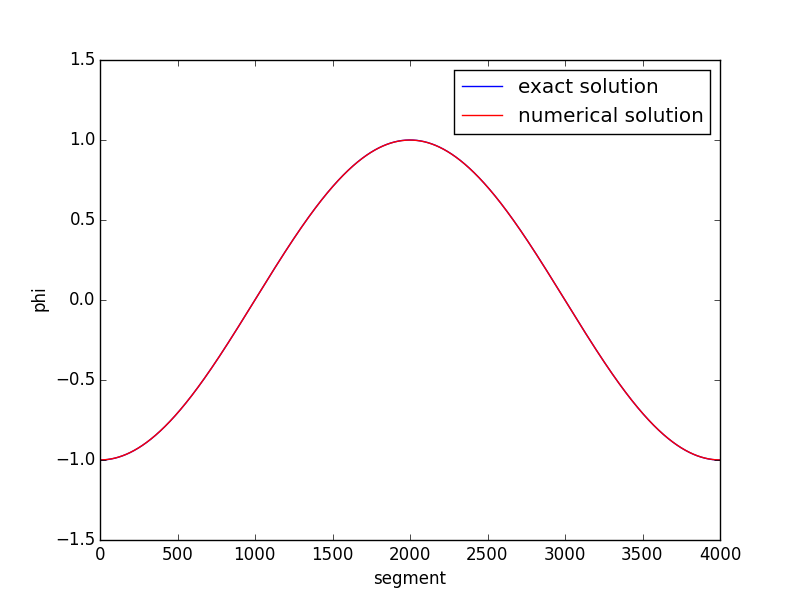
\includegraphics[scale=0.6]{exact_vs_numerical.png}
\end{figure}
\\
\newpage
The wording of the assignment puzzled me a bit, as it asked for the added mass forces, as well as the cross-coupling added mass coeeficients. If I'm not fully mistaken, the cross-coupling coefficients for symmetric 2D bodies are all zero, as well as the coefficients $m_{33}, m_{44}$ and $m_{55}$.  The added mass force is defined as $F_j = -\dot{U}m_{ji}$, but we are not given a U, so i have assumed this to be of size unity. The added mass forces would then be as follows (for the cases listed above)\\
\\
For circle: $F_1 = -3.1405\tab F_2 = -3.1405$\\
For ellipse:  $F_1 = -3.1408\tab F_2 = -12.5598\tab F_6 = -3.5315$\\
For square:  $F_1 = -4.7506\tab F_2 = -4.7506\tab F_6 = -0.723$\\
 \end{document}
